%%%%%%%%%%%%%%%%%%%%%%%%%%%%%%%%%%%%%%%%%%%%%%%%%%%%%%%%%%%%%%%%%%%%%%%%
\chapter{Neuartige modellbasierte Teststrategie für große agile Projekte basierend auf Graphwalker}
\label{sec:results}
%%%%%%%%%%%%%%%%%%%%%%%%%%%%%%%%%%%%%%%%%%%%%%%%%%%%%%%%%%%%%%%%%%%%%%%%

Aufbauend auf den Erkenntnissen der Fallstudie (siehe Abschnitt \ref{sec:fallstudie}) wurde eine neuartige modellbasierte Teststrategie entwickelt um komplexe Softwaresysteme in agilen Projekten zu testen. Diese Strategie hat unter anderem folgende Eigenschaften und zielt auf die, in Abschnitt \ref{sec:schwachstellen_raiffeisen}, beschriebenen Schwachstellen ab:

\begin{enumerate}
\item Einfachere Einbindung der Fachbereiche und Minimierung der Spezifikations-/Implementationslücke.
\item Minderung des Wartungsaufwandes für die Testlogik
\item Eliminierung der Notwendigkeit eine hohe Anzahl von einzelnen Teställen zu definieren
\item Visualisierung der Spezifikation und Bewusstmachung des potenziellen Testaufwandes
\item Minimierung der Abhängigkeit zu einem Werkzeug durch Wahl eines quelloffenen Tools
\item Möglichkeit des punktuellen Einsatzes bzw. der inkrementellen Einführung
\item Erhöhung der Testabdeckung und damit Erhöhung der Qualität des Softwaresystems
\end{enumerate}

Im folgenden wird die genannte Teststrategie näher beschrieben. Abbildung \ref{fig:testarchitektur} stellt die Testarchitektur konzeptuell dar.

\begin{figure}[h] 
  \centering
     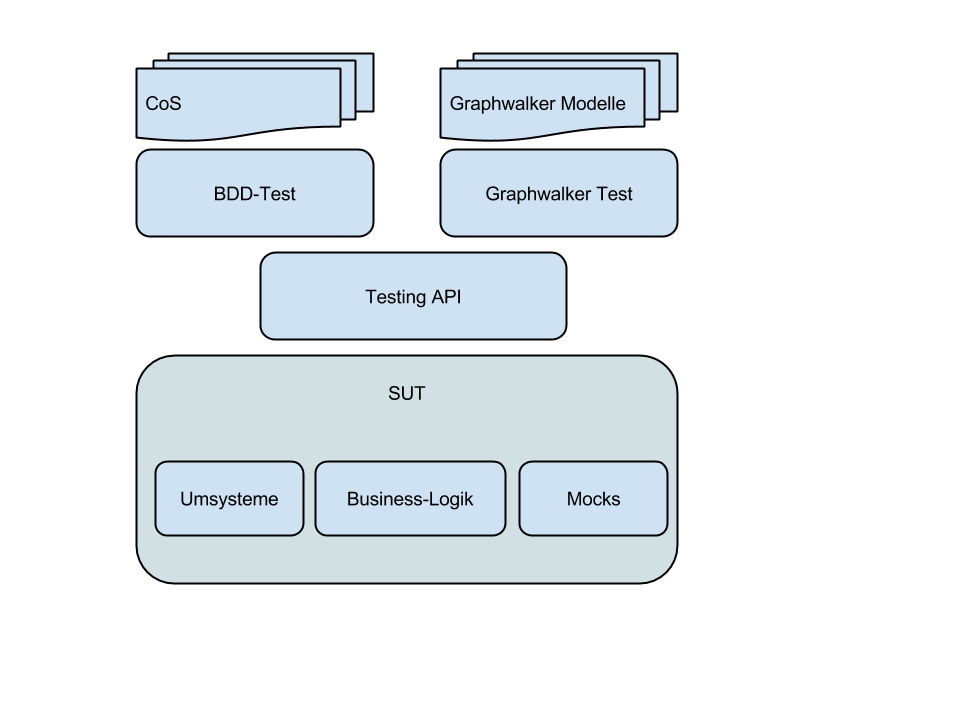
\includegraphics[width=1.0\textwidth]{figures/Testarchitektur-MBT-BDD-COS.png}
  \caption{Am oberen Ende der Testarchitektur liegen die \textit{Conditions of Satisfiction}, die vom Kunden oder Fachbereich definiert werden. Sie dienen als Basis für die BDD-Tests. Graphwalker operiert auf Modellen im graphml-Format. Dabei können beide Frameworks entweder auf die Testing API zugreifen oder direkt auf das SUT.}
  \label{fig:testarchitektur}
\end{figure}

\section{Aufbau der Teststufen}
Im Sinne von Test-First und einer hohen Priorisierung von Unit-Tests soll der Fokus des Testings auf drei Arten von Tests liegen:

\begin{itemize}
\item Eine breite Basis von Unit-Tests mit hoher Abdeckung
\item Modellbasierte Systemtests auf mehreren Ebenen mit direkter Verbindung zu Anforderungen/Changes
\item Manuelle System- und Abnahmetests
\end{itemize}

In Anlehung an Linz\cite{linz_testing_2014} (und mit dem Verweis auf die Diskussion in Abschnitt\ref{sec:discussion_unit}) soll die Unit-Test Ebene in Scrum-Projekten am breitesten sein\todo{Test PYRAMIDE einfügen}. Dies erscheint mit Hinblick auf die vielen kurzen Iterationen, die das Softwaresystem stark verändern, auch logisch. Unit-Tests lassen sich, weil sie am entwicklungsnächsten sind, auch am schnellsten modifizieren. Obwohl Unit-Tests einzelne Komponenten in Isolation testen, müssen sie zumindest eine verlässliche Aussagen treffen können, dass ebenjene Komponente ordnungsgemäß operiert. Diese Aussage wird möglich durch eine hohe Codeüberdeckung in Verbindung mit sorgfältig designten Testfällen. Auch auf Unit-Testebene gelten Best-Practices und Methodiken für hochqualitative Testfälle, wie sie Spillner und Linz beschreiben\cite{spillner_software_2014}. Die Besonderheit im Unit-Testing dieser Teststrategie liegt im Einsatz eines Behaviour-Driven-Testing\cite{chelimsky_rspec_2010} Frameworks und einer Testing-API. Für erstere Komponente existieren einige frei erhältliche Vertreter\footnote{Im Java-Umfeld bekannt sind die Frameworks \textit{jBehave} \url{http://jbehave.org/} und \textit{cucumber} \url{https://cucumber.io/}}. In der Raiffeisen-Fallstudie wurde aber eine Eigenentwicklung als \textit{Proof of Concept} gemacht (siehe Abschnitt \ref{sec:bdd} für eine kurze Erläuterung). Die erwähnte Testing-API (siehe Abschnitt \ref{sec:testing_api}) bietet Schnittstellen zu Programmlogik und Umsystemen.\\
Im Sinne dieser Arbeit steht der modellbasierte Anteil der Teststrategie im Mittelpunkt. Es soll aber erwähnt sein, dass keine zwei Softwareprojekte gleich sind und sich die Gewichtungen der Testmethodiken im Detail unterscheiden \textit{sollten}! Der modellbasierte Anteil basiert technisch ausschließlich auf quelloffenen Werkzeugen. Graphwalker (die Funktionsweise des Graphwalker-Frameworks wird in Abschnitt \ref{sec:graphwalker} erklärt) funktioniert als Testtreiber der das SUT systmatisch durchläuft. Welche bzw. welche Art von Schnittstellen in das SUT greifen und es bedienen bleibt völlig offen und muss an die eigenen Bedürfnisse angepasst werden. Bei Applikationen mit GUI (oder wenn über die GUI \textit{End-to-End} Tests gemacht werden sollen) dann könnte zum Beispiel Selenium\footnote{Webseite des Selenium-Projekts \url{http://www.seleniumhq.org/}} eingesetzt werden. Tests auf Schnittstellenebene könnten durch SoapUI\footnote{ Offizielle Webseite von SoapUI \url{http://www.soapui.org/}} oder REST-assured\footnote{Code-Repository von REST-assured \url{https://code.google.com/p/rest-assured/}} angetrieben werden. Auch mächtigere proprietäre Werkzeuge können als Teil dieser Graphwalker-Teststrategie verwendet werden, sofern sie eine Schnittstelle zum Aufruf aus Java-Code besitzen und die Ergebnisse in irgendeiner Art und Weise (bevorzugt als JUnit-Report) zurückliefern können (dieser Ansatz wurde in der Fallstudie nicht erprobt und wird deshalb nicht näher erläutert). Außerdem können Graphwalker-Modelle nicht nur Workflows darstellen die auf GUI-Ebene ablaufen. Genauso vorstellbar sind Operationen die auf Schnittstellenebenen passieren (z.B. Operationen auf Datenbanken oder Web-Services). Bei solchen Tests macht es Sinn eine stabile Zwischenschicht, die Testing-API, einzubauen die wiederrum auf die darunterliegenden Systeme zugreift. Der Aufwand zur Erstellung der API rechtfertigt sich weil auch BDD-Unit-Tests darüber in das SUT greifen.\\
Zuletzt bleiben aber auch manuelle Tests ein wichtiger Bestandteil der Teststrategie. Einerseits sind das Abnahmetests bei Neuentwicklungen beziehungsweise bei modifizierten Teilen des Systems und andererseits auch Regressionstests die geschäftskritische Teile des Systems überwachen.

\section{Details der Teststrategie und Architektur}

\subsection{Behavior Driven Testing Framework}
\label{sec:bdd}
Der Fokus dieser Arbeit liegt auf dem modellbasierten Teil der Teststrategie, trotzdem soll erläutert werden welche Rolle \textit{Behavior Driven Testing} im Gesamtbild spielt. In der Softwareentwicklung, und vor allem in großen Projekten, wird viel Aufwand betrieben um Anforderungen von Domänenexperten möglichst nahtlos in die Implementation einfließen zu lassen. Abhängig vom Projekt liegen zwischen diesen Anforderungen und der endgültigen Realisierung mehrere Stufen und Parteien. Die Einführung von BDT zielt also vor allem auf die bereits erwähnte Minimierung der Spezifikations-/Implementationslücke. Auch MBT optimiert diesen Umstand (wie in Abschnitt \ref{sec:mbt_vorteile} beschrieben), aber es hat sich herausgestellt, dass es nicht zielführend ist für jede Anforderung den modellbasierten Ansatz anzuwenden.\\
Behavior Driven Testing, im weiteren Sinne bekannt als Behavior Driven Development, wurde ursprünglich von Dan North beschrieben. Er publiziert und diskutiert über BDD auf einer von ihm verwalteten Webseite\cite{north_official_2015}. BDD basiert auf drei Grundprinzipien:

\begin{itemize}
\item Domänenexperten und Techniker sollen auf einer Ebene kommunizieren und über das System mit einem gemeinsamen Vokabular referenzieren.
\item Jedes System muss einen, für alle Parteien, klar erkennbaren unternehmerischen Wert haben. Außerdem muss bewusst werden wie dieser Wert generiert wird.
\item Allen Parteien ist bewusst, dass Analyse, Design und Spezifikation dem Ertragsgesetz unterliegen. Das heißt ab einem gewissen Punkt macht es keinen Sinn mehr Ressourcen zu investieren weil die Wertschöpfung abfällt.
\end{itemize}

Aus Sicht des Domänenexperten (im Fallbeispiel ein Bankberater und in Vertretung dessen der Fachbereich) wird eine Anforderung folgendermaßen spezifiziert: 

\begin{quote} Als \textbf{ROLLE} fordere ich \textbf{ETWAS} und gewinne dadurch \textbf{NUTZEN} \end{quote}

Diese Nähe zur fachlichen Formulierung (im gleichen Vokabular) will man in der Entwicklung nutzen um der Spezifikation so nah wie möglich zu kommen. In der Fallstudie hat sich herausgestellt, dass die erwähnten CoS-Tabellen (siehe Abschnitt \ref{sec:fallstudie}) schon recht genau solchen BDD-Anforderungen entsprechen. Auch sie beschreiben, ausgehend von einem Ausgangszustand welche Paramater zu einem bestimmten Endzustand führen sollen. Eingangs erwähnte BDD-Frameworks benutzen die selbe Struktur um Tests zu definieren. Es lag also nahe diesen Ansatz zu verfolgen, bestehende Vorgehensweisen nicht grundlegend zu verändern und gleichzeitig bessere Spezifikationen zu schaffen. Gleichzeitig bestand in der Fallstudie der Wunsch nach mehr automatischen Regressionstests die genau jene CoS prüfen. Mehrere Problemfelder wurden identifiziert die mit dem Einsatz von Behavior Driven Testing adressiert werden sollten:


\begin{itemize}
\item \textbf{Präzisierung der Spezifikation.} Spezifikationen in Prosatext und Fachjargon bieten ein hohes Potenzial für Missverständnisse und Ungenauigkeiten. Ein gemeinsames Vokabular und eine universell verständliche Syntax um diese Spezifikationen festzuhalten ist nötig.
\item \textbf{Spezifikationen müssen über lange Zeit überschaubar und prüfbar bleiben.} CoS bleiben über viele Iterationen hinweg gültig. Es kommt aber immer wieder vor, dass sie direkt angepasst werden oder von anderen Weiterentwicklungen betroffen sind und geändert werden müssen. Die von den Fachbereichen verwendeten Storybooks lassen sich zwar versionieren (mittels bekannter Dokumenten-/Codeversionierungs-Tools) aber durch die schiere Größe dieser Dokumente ist es unmöglich festzustellen welche CoS noch befriedigt sind und welche verletzt wurden. Es muss eine Form gefunden werden um CoS kompakt und versionierbar, und für alle an der Entwicklung Beteiligten verständlich, darstellen zu können.
\item \textbf{Einfache und nachhaltige Automatisierbarkeit der Regressionstests.} Aus den verfassten CoS sollen, mit wenig Aufwand, automatisierte Regressionstests entstehen. Außerdem soll der Zusatzaufwand für die Entwickler gering gehalten werden um aus den CoS automatische Regressionstests zu generieren und diese auch zu warten.
\end{itemize}

\todo{Weiter mit Beschreibung der BDD Lösung...}


\subsection{Testing API}
\label{sec:testing_api}

\subsection{Modellbasierte Tests mit Graphwalker}
























